\documentclass[11pt]{article}
\usepackage[final]{acl}
\usepackage{times}
\usepackage{latexsym}
\usepackage[T1]{fontenc}
\usepackage[utf8]{inputenc}
\usepackage{microtype}
\usepackage{inconsolata}
\usepackage{graphicx}
\usepackage{amsmath}
\usepackage{minted}
\usepackage{booktabs}

\title{\textsc{VentureTruth}: An Automated Claim Verification
Pipeline for Venture Capital Due Diligence}

\author{Yufei Yang \\
  Technical University of Munich \\
  \texttt{yufei.yang@tum.de} \\\And
  Zekai Li \\
  Technical University of Munich  \\
  \texttt{ge65kul@mytum.de} \\\AND
  Mykhailo Riabets \\
  Technical University of Munich \\
  \texttt{mykhailo.riabets@tum.de} \\\And
  Joyce Ann Clarize Galang \\
  Technical University of Munich, UVC \\
  \texttt{joyce.acdg@gmail.com}
}

\begin{document}

\maketitle

\begin{abstract}
Due diligence in venture capital involves extensive evaluation of investment opportunities. This includes going through documents and claims. This process is traditionally manual, time-consuming, and prone to inconsistencies. To address problems of the manual approach, we present \textsc{VentureTruth}, an automated end-to-end pipeline that extracts, verifies, and evaluates factual claims from startup documentation using Large Language Models (LLMs) and real-time web search. The proposed system processes input documents, extracts verifiable claims using LLM, retrieves supporting and contradictory evidence via AI-based web retrieval, and produces structured verification reports, including risk assessments of the evaluated claims. The pipeline incorporates iterative quality improvement through self-reflection of the verification results, robustness testing across prompt variations, and a suite of evaluation metrics. The results demonstrate that \textsc{VentureTruth} is able to achieve the performance of the human expert on the classification task, especially for claims that are incorrect (observed 100\% accuracy) or do not have enough validation evidence (observed more than 90\% accuracy).
\end{abstract}

\section{Introduction}

Venture capital (VC) investment decisions involve evaluating thousands of opportunities annually. Each requires rigorous due diligence (DD) to validate assertions made in pitch decks, financial models, and technical whitepapers. These claims -- ranging from investment viability to costs and potential returns -- are part of the investment thesis. Currently, verification is a labor-intensive, manual process in which analysts investigate identified claims against external knowledge sources, such as news archives, corporate filings, and industry reports.
\\
\\
This manual paradigm has the following systemic limitations. 
First, it is resource-intensive. Thoroughly verifying a single document may require multiple targeted searches and the synthesis of disparate documents. Such an approach can create a bottleneck, forcing firms to limit the depth of their diligence. 
Second, it is susceptible to inconsistency. Verification standards often vary between analysts, leading to different risk assessments of the same claim. 
Third, it does not scale. As document volume increases, the fixed capacity of human analyst teams limits the number of documents they can process.
Finally, it faces latency risks. Static diligence reports rapidly become obsolete; a manual process cannot continuously monitor for new information that might invalidate previous verification results.
\\
\\
Recent advancements in Large Language Models (LLMs) and Retrieval-Augmented Generation (RAG) offer an opportunity to automate extraction and verification processes. However, using general-purpose RAG systems for financial due diligence poses challenges. The cost of a "false positive" (hallucinating a verification) is substantially higher in an investment context. Furthermore, claims are domain-specific, requiring a deeper semantic understanding (e.g., the difference between a "signed partnership" and a "letter of intent").
\\
\\
The proposed solution is not intended as another domain-adapted RAG system. While prior work primarily optimizes for coverage or factual recall, our design targets high-stakes venture capital due diligence, where the cost of false positives can be substantial. As a result, we adopt a different perspective, treating abstention as a safety mechanism rather than a failure mode.
\\
\\
Concretely, the system enforces strict evidence independence and confidence calibration rules, prioritizing cautious verification when the corroboration is weak, dependent, or ambiguous. This logic is supposed to reflect the standards applied by the professionals, for whom an unverified claim is preferable to an incorrectly validated one. Accordingly, our solution is best understood as a calibrated decision-support architecture for high-stakes settings, rather than a generic fact-checking or question-answering pipeline. In this work, we present \textsc{VentureTruth}, an automated pipeline that bridges this gap. Unlike generic verification systems, our approach incorporates rigorous \textbf{Certainty Calibration}, \textbf{Iterative Quality Refinement}, and \textbf{Robustness Testing} to ensure that automated verdicts meet the investing standards.
\\
\\
The main contributions of this paper are as follows:
\begin{enumerate}
    \item We introduce a specialized verification logic that prioritizes safety over recall, explicitly capping confidence for single-source or dependent evidence to minimize hallucinations in investment contexts.
    \item We implement a feedback loop in which a "Quality Assessor" agent critiques verification reasoning and provides specific improvement suggestions, allowing the system to dynamically refine its search strategy.
    \item We demonstrate a method for stress-testing verdicts using "Sceptical" and "Evidence-Focused" prompt variations, ensuring that system judgments are stable and not artifacts of prompt phrasing.
    \item Beyond binary true/false verdicts, our pipeline classifies the \textit{type} and \textit{independence} of supporting evidence (e.g., differentiating between a company press release and a regulatory filing), directly mapping verification quality to investment risk.
\end{enumerate}

\paragraph{Research Questions (RQ)}. To compare the performance of the proposed solution with that of the human-like, we defined a set of research questions that will serve as the basis for the comparison.
\\
\\
\textbf{RQ1: Agreement with Expert Judgment}.
How closely do the \textsc{VentureTruth}'s verdicts correspond with human analyst annotations across the three-way label set (\texttt{SUPPORTED},\texttt{CONTRADICTED}, \allowbreak \texttt{INSUFFICIENT\_EVIDENCE})?
\\
\\
\textbf{RQ2: Calibration and Abstention under Uncertainty}.
When evidence is weak or missing, does the system appropriately abstain (i.e., predict \texttt{INSUFFICIENT\_EVIDENCE}) and avoid overconfident decisions compared to human baselines?

\paragraph{Author Contributions.}
Mykhailo initiated the project by establishing the initial codebase structure and implementing the search engine module.
Yufei led the claim extraction component and designed the overall system architecture, including the quality-checking pipeline and the testing framework.
Zekai further modularized the codebase and refactored the system into an iterative workflow to enable repeated refinement and evaluation.
\section{Related Literature}
Our work combines concepts from automated fact-checking, search-based verification, RAG, and LLM-based self-refinement and introduces a novel application of AI in venture capital due diligence. In the following, we will review each area and explain our contributions.
\\
\\
\textbf{Automated fact-checking.} The task of factual claims verification has been studied extensively in NLP. \citet{guo2022survey} provides a comprehensive survey defining a three-stage pipeline: claim detection, evidence retrieval, and veracity prediction. Subsequent work extended verification to structured data \citep{aly2021feverous} and real-world web claims \citep{schlichtkrull2024averitec}. Two recent surveys document the shift toward LLM-based approaches. \citet{dmonte2025claim} examines how RAG and prompting strategies are reshaping claim verification pipelines, while \citet{vykopal2024generative} focuses specifically on LLMs across all stages of fact-checking. Our work follows the general pipeline structure but targets a novel domain -- venture capital due diligence -- where claims are domain-specific, unverifiable through standard knowledge bases, and must be linked to investment risk.
\\
\\
\textbf{Search-based verification.} Several systems have combined LLMs with external tools for factuality assessment. FacTool \citep{chern2023factool} proposes a task-agnostic framework that extracts claims from LLM-generated text, generates search queries, gathers evidence via Google Search and other tools, and verifies each claim. SAFE \citep{wei2024longform} takes a similar approach to evaluating long-form factuality, decomposing responses into atomic facts and verifying each using multi-step Google Search reasoning. OpenFactCheck \citep{wang2024openfactcheck} provides a modular framework that allows claim processors, retrievers, and verifiers to be freely combined and configured. Our pipeline uses search-based verification similar to FacTool and SAFE. However, unlike these systems, which primarily verify LLM-generated text or political claims, \textsc{VentrureTruth} targets structured business documents and connects verification outcomes to the risk assessments.
\\
\\
\textbf{RAG.} RAG has become a dominant paradigm for grounding LLM outputs in external knowledge \citep{gao2023retrieval}. By retrieving relevant documents before generation, RAG systems reduce hallucinations and enable access to the latest information. \citet{adjali2024exploring} applies RAG specifically to the AVeriTeC real-world claim verification shared task, integrating dense retrieval with question generation in an end-to-end setup. In our system, we use Perplexity's Sonar Pro model as a search-augmented retriever that queries the internet, ensuring that verification evidence reflects the most current publicly available information.
\\
\\
\textbf{LLM-based self-refinement.} \citet{madaan2023selfrefine} introduces Self-Refine, demonstrating that LLMs can iteratively improve their outputs through a feedback-refine loop without additional training. \citet{shinn2023reflexion} propose Reflexion, where language agents use verbal self-reflection and dynamic memory to improve task performance over successive attempts. Our pipeline incorporates a similar self-reflection mechanism: after initial claim verification, the system reviews its own outputs for completeness and consistency, iteratively refining verification results.
\\
\\
\textbf{AI in venture capital due diligence.} While commercial tools such as Caena, Tracxn, and AlphaSense have begun integrating AI for deal sourcing, document review, and financial analysis, there is limited academic work specifically addressing automated claim verification in the context of startup evaluation. Existing tools focus primarily on data aggregation and pattern recognition rather than end-to-end factual verification of specific claims made in pitch materials. \textsc{VentureTruth} addresses this gap by providing a transparent, traceable pipeline that extracts individual claims from startup pitch documents, verifies each against web sources, and produces structured risk assessments for investor decision-making.

\section{Methodology}
\subsection{Definitions}
Before we explain our approach to solve the problem, explained in the Introduction section, we have to make definitions used in the following parts.
\subsubsection{Claim}
We define a claim $c$ as an atomic, factual assertion extracted from a startup’s documentation $D$ (e.g., pitch decks, reports, and supplementary materials). A valid claim must satisfy the following properties:
\begin{enumerate}
    \item \textbf{Verifiability:} It can be supported or refuted by external evidence.
    \item \textbf{Atomicity:} It expresses a single verifiable proposition; compound statements are decomposed.
    \item \textbf{External-facing:} It refers to an objective state of the world (e.g., partnerships, regulatory status, deployments) rather than intent or promotional language.
\end{enumerate}
Each claim is assigned a unique identifier and stored with provenance (document name, page, or section) for traceability.

\subsubsection{Evidences and Verdicts}
For each claim $c$, the system retrieves external evidences $E=\{e_1,\dots,e_n\}$ from the public information sources and outputs a verdict $L \in \{$\texttt{SUPPORTED}$,\texttt{CONTRADICTED}, \allowbreak \texttt{INSUFFICIENT\_EVIDENCE}\}$ with confidence score $s \in [0,1]$. A more detailed explanation of the scoring system can be found in Appendix \ref{appendix:classification_rules}. 
\\
\\
For each evidence item $e$, the following information is assigned:
\begin{itemize}
    \item a source tier $\textsc{Tier}(e) \in \{\texttt{Regulatory}, \texttt{News},\allowbreak \texttt{Industry}, \texttt{Official}, \allowbreak \texttt{Social}, \texttt{Other}\}$,
    \item an independence flag $\textsc{Independent}(e,c)$ indicating organizational independence from the claiming entity (e.g., company websites and press releases in \texttt{Official} are dependent).
\end{itemize}
~\\
The verdicts \texttt{SUPPORTED}, and \texttt{CONTRADICTED} require at least one independent evidence item from the \texttt{Regulatory}, \texttt{News}, or \texttt{Industry} tiers; otherwise, the system defaults to \texttt{INSUFFICIENT\_EVIDENCE}. The formal verdict definitions used by \textsc{VentureTruth} are:
\begin{itemize}
    \item \textbf{SUPPORTED:} $\exists e \in E : \textsc{Entails}(e,c) \land \textsc{IsReliable}(e)$.
    \item \textbf{CONTRADICTED:} $\exists e \in E : \textsc{Contradicts}(e,c) \land \textsc{IsReliable}(e)$.
    \item \textbf{INSUFFICIENT\_EVIDENCE:} is applied when (i) no relevant evidence is retrieved, (ii) only dependent/self-published or low-credibility evidence exists, or (iii) evidence is inconclusive.
\end{itemize}
~\\
If both reliable entailment and contradiction signals exist, the system outputs \texttt{CONTRADICTED} when contradictory evidence is of equal or greater reliability than supporting evidence. Otherwise, it outputs \texttt{INSUFFICIENT\_EVIDENCE} and flags an evidence conflict.

\subsection{System Architecture}

\begin{figure}[htpb]
    \centering
    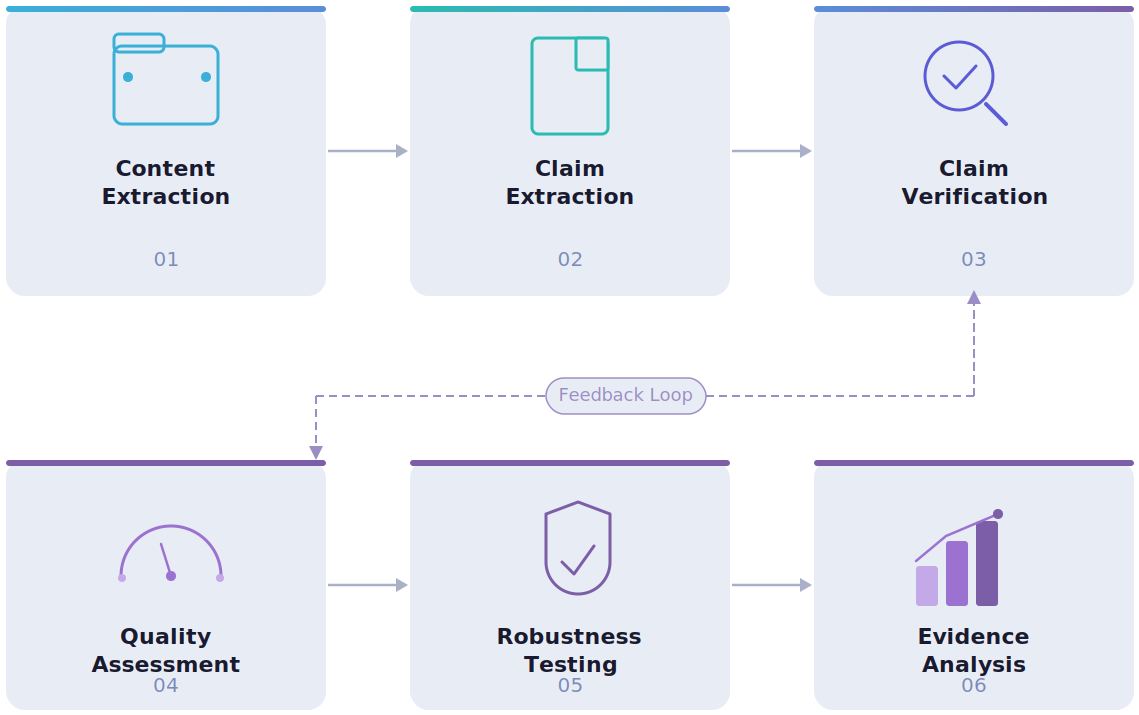
\includegraphics[width=\linewidth]{resources/venture_truth_architecture_light_larger_font.png}
    \caption{The \textsc{VentureTruth} pipeline architecture.}
    \label{fig:venture_truth_structure}
\end{figure}

As illustrated in Figure~\ref{fig:venture_truth_structure}, \textsc{VentureTruth} comprises six modules: \textit{Content Extraction}, \textit{Claim Extraction}, \textit{Claim Verification}, \textit{Quality Assessment}, \textit{Robustness Testing}, and \textit{Evidence Analysis}. Below, we summarize the purpose of each component.
\\
\\
\textbf{Content Extraction.} This module ingests raw materials (e.g., PDFs) and structured metadata (e.g., CSVs) and produces a unified representation. It combines standard PDF parsing with OCR to support both digitally encoded and scanned, image-heavy documents.
\\
\\
\textbf{Claim Extraction.} This module identifies atomic, external-facing factual claims while filtering out subjective or promotional statements. Compound claims are decomposed to ensure one-to-one correspondence between claims and verifiable propositions.
\\
\\
\textbf{Claim Verification.} For each claim, the verifier retrieves web evidence and outputs a verdict with confidence according to the predefined rules. Verification is embedded in an iterative refinement loop that incorporates feedback from the quality assessment component.
\\
\\
\textbf{Quality Assessment.} This module critiques verification outputs along three dimensions: reasoning soundness, source relevance/independence, and confidence calibration. It produces structured feedback (e.g., refining queries, resolving entity aliases, tightening evidence thresholds) that is injected into subsequent verification iterations.
\\
\\
\textbf{Robustness Testing.} This module re-verifies claims under prompt variations (neutral, evidence-focused, sceptical) and measures verdict agreement and confidence variance. Unstable claims are flagged for abstention or manual review.
\\
\\
\textbf{Evidence Analysis.} This module categorizes sources (news, regulatory, industry, official, social, other) and computes evidence diversity (e.g., unique domains per claim) to analyze how evidentiary breadth relates to model confidence. This is the last step of the pipeline that produces the final output. Sample output of the pipeline can be found in Appendix \ref{appendix:sample_output}.

\subsection{Implementation Details}
The \textsc{VentureTruth} pipeline is implemented in Python and parametrized via a single YAML configuration that specifies paths, model parameters, and operational thresholds.
\\
\\
\textbf{Content Extraction.} The ingestion phase aggregates metadata from \texttt{csv\_path} and documents from \texttt{pdf\_folder}. It uses \texttt{PyPDF2} for standard text extraction and \texttt{pdf2image} and \ texttt {pytesseract} for text extraction from images. The extracted data is matched against the metadata and stored as structured JSON, combining metadata and document text.
\\
\\
\textbf{Claim Extraction.} It uses an LLM to generate candidate claims with unique identifiers and a claim-confidence score. Prompts enforce atomicity, falsifiability, and external-facing relevance. To minimize model hallucination, we set the temperature to 0.
\\
\\
\textbf{Claim Verification.} Verification is managed by a \texttt{SearchManager} and \texttt{ClaimVerifier}.
\\
\\
The \texttt{SearchManager} queries the Perplexity API (\texttt{sonar-pro}) and performs:
\begin{enumerate}
    \item \textbf{Entity resolution:} identify the primary entity and aliases (e.g., legal vs.\ brand names);
    \item \textbf{Multi-angle querying:} target (a) official announcements, (b) independent journalism, and (c) regulatory/third-party registries;
    \item \textbf{Result triage:} label URLs by relevance (\texttt{HIGH, MEDIUM, LOW, OFF\_TOPIC}) and retain top results.
\end{enumerate}
~\\
The \texttt{ClaimVerifier} invokes an LLM at temperature 0 to output a structured verdict and confidence score, following calibration rules:
\begin{itemize}
    \item \texttt{INSUFFICIENT\_EVIDENCE}: triggered when evidence is absent, dependent/self-published, or inconclusive; confidence is bounded to a score range of $0.3$ -- $0.5$.
    \item \texttt{SUPPORTED}: requires independent corroboration; high confidence ($>0.8$) requires at least two robust independent sources.
    \item \textbf{Source independence:} entity websites and press releases are treated as dependent and are insufficient alone for high-confidence support.
\end{itemize}
~\\
\textbf{Quality Assessment.} The \texttt{QualityChecker} uses a LLM (temperature 0.1) to critique preliminary reports and assigns continuous scores in $[0,1]$ for Reasoning Quality, Source Relevance/Independence, and Certainty Calibration. Scores are discretized into \texttt{EXCELLENT}, \texttt{GOOD}, \texttt{ACCEPTABLE}, \texttt{POOR}, or \texttt{CRITICAL}. If ratings fall below the threshold, the system generates targeted recommendations that guide a subsequent verification iteration.
\\
\\
\textbf{Robustness Testing.} The \texttt{RobustnessChecker} re-verifies claims across neutral, evidence-focused, and sceptical prompts and tracks verdict agreement and confidence variance. Claims with agreement below a threshold of $<0.67$ or high variance are flagged as unstable, triggering forced abstention or manual review.
\\
\\
\textbf{Evidence Analysis.} The \texttt{ClaimsEvidence\allowbreak Analyzer} assigns sources to \texttt{News}, \texttt{Regulatory}, \texttt{Industry}, \texttt{Official}, \texttt{Social}, and \texttt{Other} via URL/domain heuristics and computes descriptive statistics (e.g., number of sources and unique domains per claim) to analyze the relationship between evidentiary diversity and confidence.
\section{Results}

\subsection{Experimental Setup}
To ensure reproducibility, we summarize the experimental configuration used to produce the results reported in Section 4.2.
\\
\\
To answer formulated research questions, we evaluate on a set of 42 claims annotated by domain professionals (18 \texttt{SUPPORTED}, 22 \texttt{INSUFFICIENT\_EVIDENCE}, 2 \texttt{CONTRADICTED}). The claims were generated by our pipeline from the input company materials and then independently labelled by experts following the guidelines in Appendix~\ref{appendix:classification_rules}. Each claim is assigned to one of three classes (\texttt{SUPPORTED}, \texttt{INSUFFICIENT\_EVIDENCE}, \texttt{CONTRADICTED}) and accompanied by a confidence score $s \in [0,1]$ reflecting the annotator's perceived evidential strength. This level of expert, fine-grained assessment is more expensive than large-scale crowdsourcing, but it better matches the real-world decision setting in which claims are reviewed under stringent privacy constraints.
\\
\\
Main components of \textsc{VentureTruth} have their own configuration. In the following, we will briefly describe the configuration used for each of them. For \textbf{Content Extraction}, the only task-relevant parameter is \texttt{limit}, which we set to 14, yielding 42 candidate claims for the subsequent step.
\\
\\
For \textbf{Claim Extraction}, we set \texttt{max\_claims} to 3. The extractor LLM was configured with \texttt{model} = \texttt{gpt-5.2} and \texttt{temperature} = 0 to ensure deterministic structured outputs.
\\
\\
For \textbf{Claim Verification}, we used \texttt{model} = \texttt{gpt-5.2} with \texttt{temperature} = 0.
\\
\\
For the \textbf{Quality Checker}, we used \texttt{model} = \texttt{gpt-5.2} with \texttt{temperature} = 0.1 to allow limited variability for critique generation while keeping the evaluation stable.
\\
\\
For the \textbf{Robustness Testing} and \textbf{Evidence Analysis}, we do not have global configuration in our pipeline.

\subsection{Measurements}

\begin{figure}
    \centering
    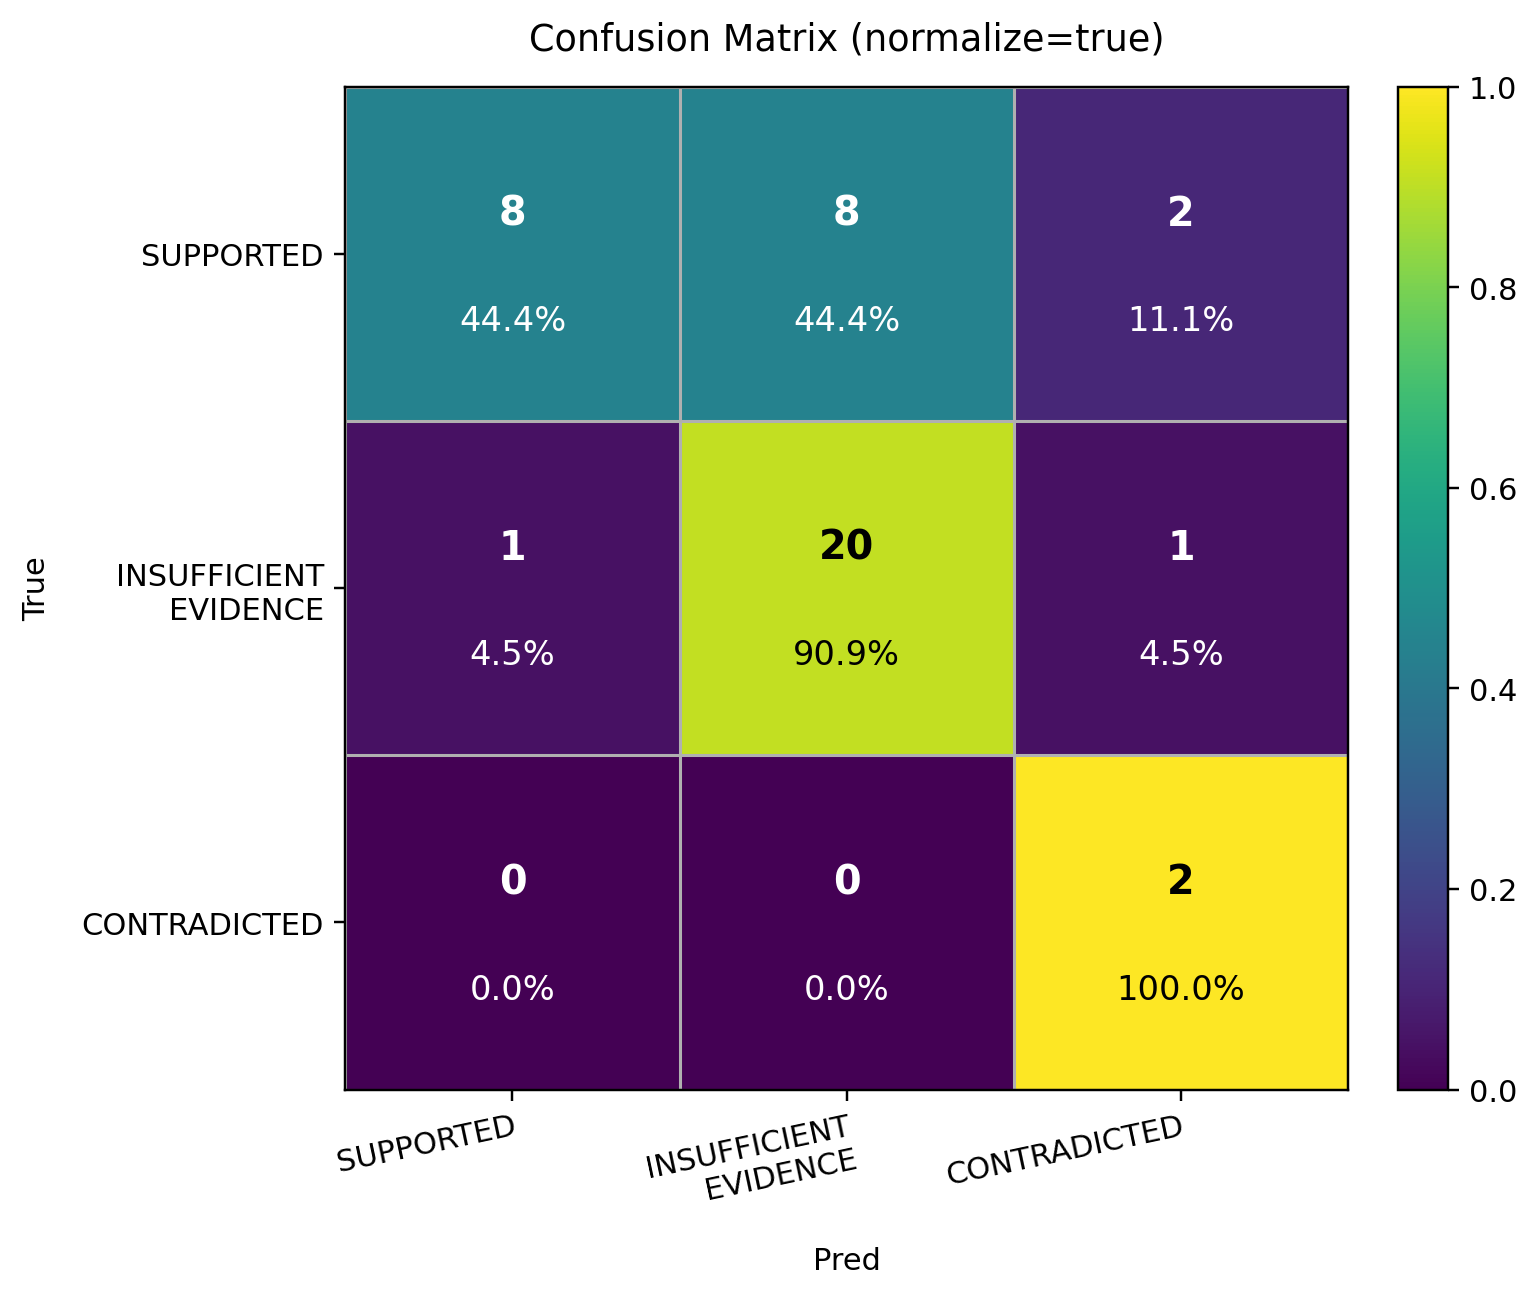
\includegraphics[width=\linewidth]{resources/confusion_matrix.png}
    \caption{\textsc{VentureTruth} confusion matrix}
    \label{fig:confusion}
\end{figure}

Per-class classification outcomes are shown in Figure~\ref{fig:confusion}, where the x-axis denotes \textsc{VentureTruth} predictions and the y-axis the ground-truth labels. The pipeline correctly identifies all \texttt{CONTRADICTED} claims. Performance is similarly strong on \texttt{INSUFFICIENT\_EVIDENCE}: \textsc{VentureTruth} correctly predicts 90.8\% of these cases. In contrast, performance on \texttt{SUPPORTED} claims is substantially lower. A majority (55.5\%) of ground-truth \texttt{SUPPORTED} claims are instead predicted as \texttt{CONTRADICTED} or \texttt{INSUFFICIENT\_EVIDENCE}, yielding only 8 correct predictions out of 18.

\begin{figure}
    \centering
    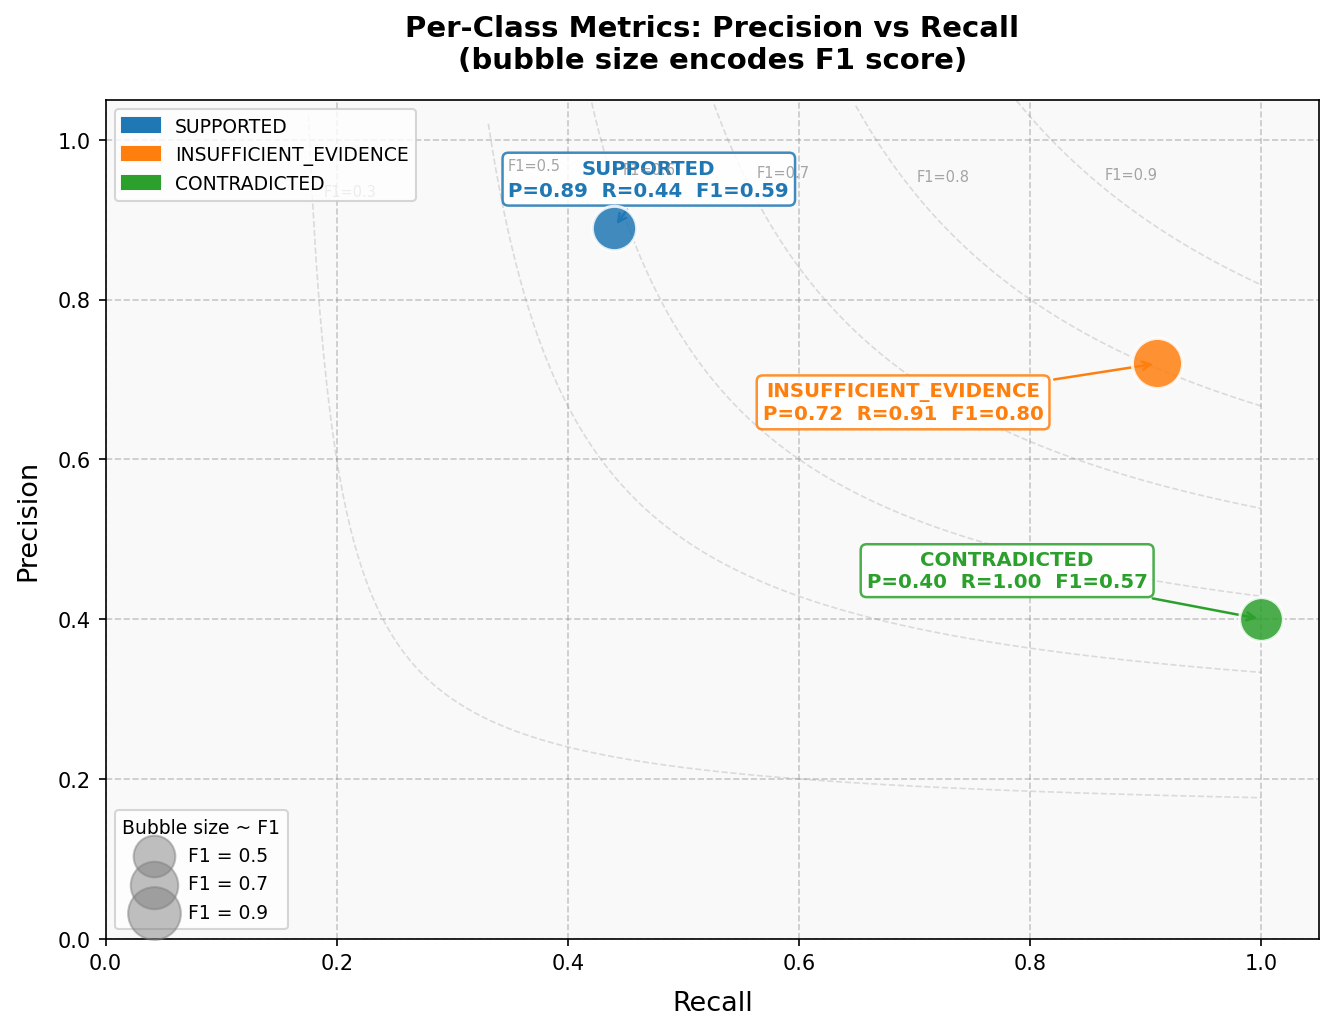
\includegraphics[width=\linewidth]{resources/f1_recall_precision.png}
    \caption{Per-class precision recall and F1-score}
    \label{fig:f1_precision_recall}
\end{figure}

~\\
According to Figure~\ref{fig:confusion}, we compute per-class precision, recall, and F1-score. The results are visualized in Figure~\ref{fig:f1_precision_recall}. Recall is shown on the x-axis, precision on the y-axis, and bubble size encodes the F1-score. For \texttt{CONTRADICTED}, the model attains a precision of 0.40 and a recall of 1.00, corresponding to an F1-score of 0.57. For \texttt{SUPPORTED}, we observe high precision (0.89) but substantially lower recall (0.44), yielding an F1-score of 0.59. Finally, \texttt{INSUFFICIENT\_EVIDENCE} achieves both strong precision (0.72) and recall (0.91), resulting in the highest F1-score of 0.80.
\section{Discussion}

\subsection{Interpretation of Results}
The experimental results represent design decisions of the \textsc{VentureTruth}. Namely, it is designed to avoid false positives.
The confusion matrix (Figure \ref{fig:confusion}) reveals a strong bias towards "conservative" verdicts (\texttt{INSUFFICIENT\_EVIDENCE} and \texttt{CONTRADICTED}). This behaviour is a direct consequence of our verification rules~(Appendix \ref{app:claim_verification}), which explicitly limit confidence scores ($<0.7$) for claims supported by only a single source or dependent evidence.
\\
\\
For the \texttt{SUPPORTED} class, high precision (89\%) and moderate recall (44\%) reflect the model's behaviour as a strict filter during the verification stage. Therefore, it may discard valid claims if the retrieval step fails to find multiple independent sources.
\\
\\
The \texttt{INSUFFICIENT\_EVIDENCE} class achieves the highest recall and precision. The high recall here indicates that the system correctly identifies claims that cannot be verified using the provided sources. Whereas, high precision means that \textsc{VentureTruth} has a low chance of classifying an invalid or correct claim as one that cannot be verified.
\\
\\
For the \texttt{CONTRADICTED} class, our model shows perfect recall (identifying all actual contradictions) but lower precision (40\%). This observation suggests that the model is sensitive to conflicting signals. In addition, such a difference can be explained by class imbalance.
\\
\\
Therefore, we can state that our pipeline achieves performance comparable to that of human experts for the \texttt{CONTRADICTED} and \texttt{INSUFFICIENT\_EVIDENCE} claims. However, it performs weakly with the \texttt{SUPPORTED} claims. This is the answer for RQ1.
\\
\\
We also observed that \textsc{VentureTruth} misclassified almost half of the supported claims. This indicates that the model was unsure about the source credibility. This means the system abstains when unsure, which answers RQ2.

\subsection{Limitations}
Our study faces several limitations that contextualize these findings:
\begin{enumerate}
    \item \textbf{Dataset Scale \& Imbalance:} The evaluation was conducted on a set of 42 annotated claims. Thus, the observed results cannot be generalized. Moreover, the class distribution of the test data is another important limitation. For the \texttt{CONTRADICTED} class, we had only 2 samples, which limits the pipeline's evaluation quality for that class.
    \item \textbf{Source Accessibility:} The current pipeline relies exclusively on the web search. It cannot access private information sources like paid registries, court filings, and private deal databases, leading to \texttt{CONTRADICTED} or \texttt{INSUFFICIENT\_EVIDENCE} verdicts for truthful claims that lack public footprints.
    \item \textbf{Model selection:} Our experiments primarily utilized the OpenAI GPT-5.2 model. While performant, relying on a single model family may introduce specific biases in reasoning.
\end{enumerate}

\subsection{Future Research Directions}
To address these limitations and further enhance \textsc{VentureTruth}, we formulated the following directions:
\\
\\
\textbf{1. Advanced Reasoning Architectures}. To address the precision/recall trade-off, future work should move beyond simple RAG to a Chain of Verification (CoVe) approach. This would split the verification process into distinct "Plan", "Execute", and "Verify" steps, allowing the system to decompose complex claims into sub-questions and verify them independently before synthesizing a final verdict.
\\
\\
\textbf{2. Constitutional AI for Calibration}. Currently, our quality assessment relies on prompt engineering. adopting a \textbf{Constitutional AI} framework would involve training or fine-tuning a "Critic" model on a dataset of correctly calibrated verdicts (e.g., "Always reject single-source support"). This would enforce our calibration rules more reliably than prompt instructions alone.
\\
\\
\textbf{3. Multi-Agent Adversarial Debate}. To enable more nuanced verdicts, we propose a multi-agent system where a "Proponent" agent and a "Sceptic" agent debate the validity of a claim. A "Judge" agent would then arbitrate. This adversarial setup could reduce confirmation bias and better simulate the collaborative nature of a human investment committee.
\\
\\
\textbf{4. Hybrid Information Retrieval}. Expanding the ingestion pipeline to support trusted, structured data sources (e.g., the Crunchbase API, localized corporate registries) would reduce false negatives for private-market claims that are not present in free search engines.


\section{Conclusion} \textsc{VentureTruth} demonstrates the viability of automating factual claim verification within venture capital due diligence. By integrating structural claim extraction, retrieval-augmented verification, and quality assessment, the pipeline delivers scalable, consistent claim analysis grounded in traceable sources. Consequently, this automated approach significantly accelerates the verification phase, enabling human analysts to concentrate on more complex cases. However, while \textsc{VentureTruth} provides robust evidentiary support, human judgment remains an important component of the final investment decision.

\bibliography{bibiliography}

\appendix

\section{Appendix}

\subsection{Sample Output}
\label{appendix:sample_output}
\begin{minted}[fontsize=\small, frame=single, breaklines]{JSON}
{
  "claim_id": "C1",
  "claim_text": "X is a startup based in Germany.",
  "category": "other",
  "extraction_confidence": 0.95,
  "original_evidence": "'Startup Country': 'Germany'",
  "verification": {
    "verdict": "SUPPORTED",
    "certainty": 0.9,
    "reasoning": "Multiple independent third-party company/startup directories and profiles consistently list X's headquarters/location as Berlin, Germany. The company's own website also references Brandbrandnew GmbH and indicates operations ended, which aligns with the existence of a Germany-based startup entity.",
    "evidence_type": "consistent_sources",
    "source_count": 7,
    "sources": [
      "https://www.cbinsights.com/company/X",
      "https://startup-map.cologne/companies/X/t
      eam/alumni-founders",
      "https://www.startupnight.net/
      startups/2023/hX",
      "https://www.startbas
      e.com/organization/X/"
    ],
    "contradiction_details": null
  },
  "risk_assessment": {
    "risk_level": "low",
    "investor_alert": false,
    "requires_followup": false,
    "followup_questions": []
  }
}
\end{minted}


% =====================================


\subsection{Classification rules}
\label{appendix:classification_rules}

\begin{table*}[t]
\centering
\renewcommand{\arraystretch}{1.4}
\begin{tabular}{@{}p{0.2\linewidth} p{0.75\linewidth}@{}}
\toprule
\textbf{Annotation Field} & \textbf{Criteria and Rules} \\ 
\midrule

\multicolumn{2}{@{}l}{\textbf{1. Verdict Assignment ($L$)}} \\
\midrule
\texttt{SUPPORTED} & 
\textbf{Condition:} The retrieved evidence $E$ explicitly confirms or clearly entails the claim. \\
& \textbf{Rule:} Must be backed by at least one independent, high-reliability source (e.g., \texttt{Regulatory}, \texttt{News}, \texttt{Industry}). Statements found \textit{only} on the company's official channels (\texttt{Official}) cannot yield a \texttt{SUPPORTED} verdict on their own. \\

\texttt{CONTRADICTED} & 
\textbf{Condition:} The retrieved evidence $E$ explicitly refutes or clearly contradicts the claim. \\
& \textbf{Rule:} If evidence conflicts, the refuting evidence must be of equal or greater reliability than the supporting evidence to assign this label. \\

\texttt{INSUFFICIENT\_} & 
\textbf{Condition:} A definitive conclusion cannot be drawn from the available evidence. \\
\texttt{EVIDENCE} & \textbf{Rule:} Assign this label if: (i) no relevant evidence is found, (ii) evidence is entirely dependent or self-published (\texttt{Official}), (iii) evidence is vague or low-credibility (\texttt{Social}), or (iv) an unresolvable conflict exists among equally reliable sources. \\

\midrule
\multicolumn{2}{@{}l}{\textbf{2. Confidence Scoring ($s \in [0,1]$)}} \\
\midrule
\textbf{High Certainty} \newline ($0.8 \le s \le 1.0$) & 
\textbf{Condition:} The verdict is indisputable based on the available evidence. \\
& \textbf{Rule for \texttt{SUPPORTED}/\texttt{CONTRADICTED}:} Requires corroboration from multiple (at least two) independent, top-tier sources. \\

\textbf{Moderate Certainty} \newline ($0.5 < s < 0.8$) & 
\textbf{Condition:} The verdict is highly probable, but the evidence lacks perfect redundancy. \\
& \textbf{Rule:} Backed by exactly one independent, reliable source, or slightly ambiguous wording that leans strongly in one direction. \\

\textbf{Low Certainty} \newline ($0.0 \le s \le 0.5$) & 
\textbf{Condition:} The verdict is forced due to evidentiary weakness or severe ambiguity. \\
& \textbf{Rule:} This range is essentially reserved for \texttt{INSUFFICIENT\_EVIDENCE} verdicts, reflecting cautious abstention. \\
\end{tabular}
\caption{Annotation guidelines and rules for human claim evaluation. Evaluators assess each claim based on the retrieved evidence $E$ and assign a verdict $L$ along with a confidence score $s \in [0,1]$.}
\label{tab:annotation_rules}
\end{table*}

% ----------------------------------------------
\section{Primary System Prompts and Core Thresholds}
\label{app:prompts_thresholds}

VentureTruth's AI modules are driven by specialized prompts designed to enforce analytical rigor and conservative calibration. This appendix documents the core prompt intents together with the \emph{exact} thresholds and deterministic rules enforced throughout the pipeline.

\subsection{Claim Extraction}
\label{app:claim_extraction}

\textbf{Goal.} Extract verifiable marketing and factual claims from raw text.

\textbf{Filtering Rules.} The extraction prompt enforces strict exclusion of:
(i) funding goals and fundraising targets,
(ii) intentions and forward-looking statements (e.g., ``We plan to \dots''),
(iii) subjective opinions and value judgments, and
(iv) internal-only metadata (e.g., generic team sizes without external corroboration).
Compound factual statements (e.g., ``We partnered with X and grew Y\%'') are decomposed into distinct atomic claims.

\textbf{Limits and Decoding.} The extractor is configured to output between 3 and 20 claims per company (configurable), with a default maximum of 3 claims in the deployed configuration. Decoding is deterministic with temperature $T=0$.

\subsection{Evidence Retrieval (Search Manager)}
\label{app:evidence_retrieval}

\textbf{Goal.} Retrieve diverse, highly relevant public sources that may corroborate or refute extracted claims.

\textbf{Retrieval Settings.} Evidence retrieval uses Perplexity's \texttt{sonar-pro} API with a 60-second timeout and a maximum of 500 generated tokens per API call.

\textbf{Search Process.} The search prompt instructs the model to generate multi-angle queries (e.g., official, news, financial, and industry perspectives) to maximize coverage, targeting 5--10 distinct sources per claim.

\textbf{Quality Assessment and Retries.} Retrieval quality is evaluated on an ordinal scale from \textsc{FAILED} to \textsc{EXCELLENT}, where \textsc{EXCELLENT} corresponds to five or more highly relevant sources. If a retrieval attempt is rated \textsc{FAILED}, the system triggers exactly one automatic retry (maximum retries: 1) with forced query reformulation.

\subsection{Claim Verification}
\label{app:claim_verification}

\textbf{Goal.} Assess each claim against retrieved evidence and assign a verdict
$y \in \{\texttt{SUPPORTED}, \texttt{CONTRADICTED}, \texttt{INSUFFICIENT\_EVIDENCE}\}$.

\textbf{Certainty Output.} The verifier returns a calibrated certainty score $c \in [0,1]$ alongside the verdict.

\textbf{Strict Certainty Thresholds.} The system enforces the following hard constraints:
\begin{itemize}
    \item \textbf{No evidence found:} $c \le 0.3$.
    \item \textbf{Internal-only reference:} if evidence consists solely of internal material (e.g., an internal pitch deck) without public corroboration, the verdict is forced to \texttt{INSUFFICIENT\_EVIDENCE} and $c \le 0.4$.
    \item \textbf{Single source / interdependent sources:} $c \le 0.7$.
    \item \textbf{High confidence:} $c \ge 0.8$ requires at least two independent primary sources.
\end{itemize}

\textbf{Independence Definition.} Official website pages, press releases, and founder interviews are explicitly classified as \emph{dependent} sources and cannot be used alone to justify high-confidence support.

\subsection{Quality Assessment (Critic)}
\label{app:critic}

\textbf{Goal.} Critically evaluate verification iterations and produce feedback to guide iterative refinement.

\textbf{Settings.} The critic module is executed via \texttt{gpt-5.2-pro} with temperature $T=0.1$ for consistent analytical feedback.

\textbf{Structured Scoring.} The critic assigns continuous scores in $[0,1]$ along three dimensions:
\begin{enumerate}
    \item \emph{Reasoning Quality:} whether the reasoning is logically sound;
    \item \emph{Source Relevance:} whether sources are credible and independent;
    \item \emph{Certainty Calibration:} whether the reported certainty matches the enforced thresholds.
\end{enumerate}

\textbf{Output Categories and Actions.} Scores are mapped to five qualitative categories:
\textsc{EXCELLENT}, \textsc{GOOD}, \textsc{ACCEPTABLE}, \textsc{POOR}, and \textsc{CRITICAL}.
If the critic detects systematic failure modes, it outputs explicit action items (e.g., ``exclude press releases''), which are enforced in the subsequent iteration.

\subsection{Robustness Testing Variations}
\label{app:robustness}

\textbf{Goal.} Test verdict stability across different analytical personas and flag unstable verifications.

\textbf{Agreement Threshold.} A verification is flagged as unstable and may be forced to \texttt{INSUFFICIENT\_EVIDENCE} if the inter-variation agreement rate is below $0.67$ (e.g., fewer than two agreeing verdicts out of three prompt variations).

\textbf{Prompt Personas.} Robustness testing uses three prompt variants:
\begin{itemize}
    \item \textbf{Neutral (Default):} balanced verification under the standard rules above.
    \item \textbf{Evidence-Focused:} \texttt{SUPPORTED} requires $\ge 3$ independent high-quality sources; fewer than two sources default to \texttt{INSUFFICIENT\_EVIDENCE}.
    \item \textbf{Skeptical:} default stance is doubt; high confidence requires $\ge 4$ independent sources, and single-source verifications are penalized with $c \le 0.4$.
\end{itemize}

\subsection{Metadata Evaluation}
\label{app:metadata_eval}

Pipeline-extracted corporate metadata is validated against CRM ground truth (Salesforce) using token-level fuzzy string matching. A strict similarity threshold of $0.85$ is applied to tolerate benign lexical variations (e.g., ``Inc.'' vs.\ ``Incorporated''). Matching performance is reported using precision and recall.


% ================================



\end{document}
